\section{Architecture}
\label{sec:architecture}

The system architecture can be visualized in the Figure \ref{fig:architecture}
below, and it illustrates how each entity of the project interacts with each
other, taking into account the requirements mentioned in the previous Sections.

\begin{figure}[H]
    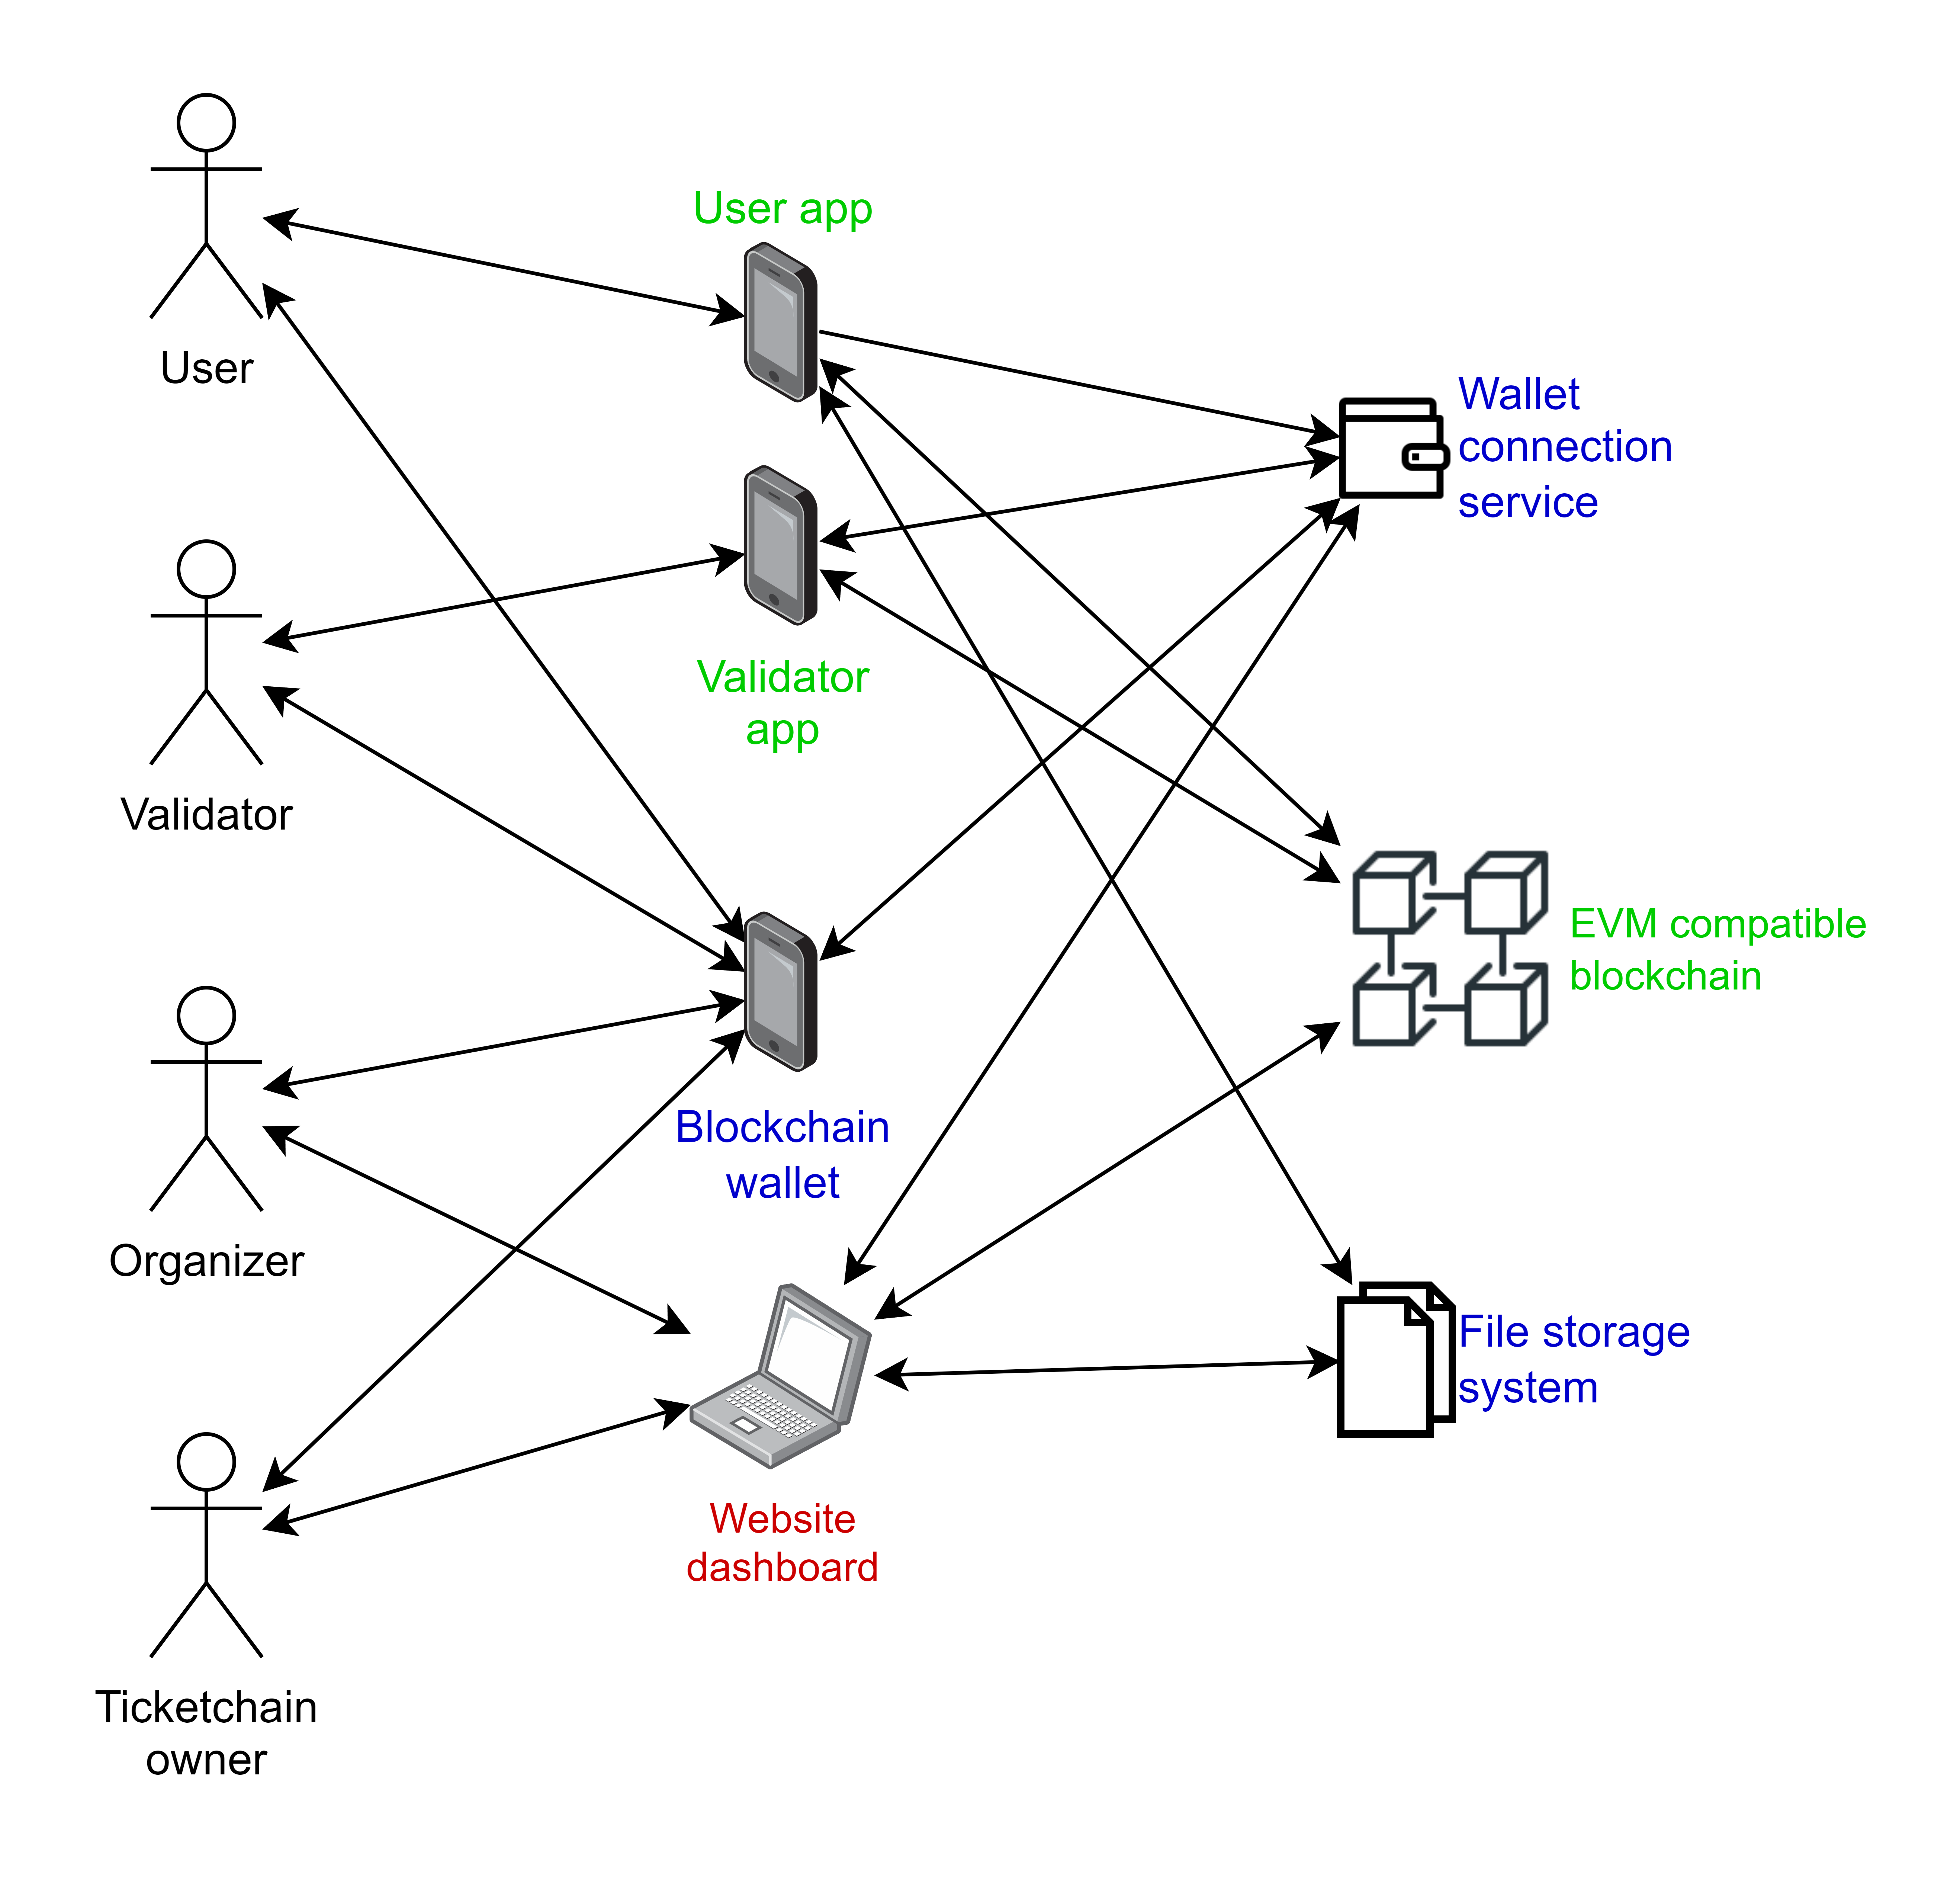
\includegraphics[width=\textwidth*2/3]{Architecture.png}
    \centering
    \caption{Architecture}
    \label{fig:architecture}
\end{figure}

We will have a mobile application for both common users and validators and a
website dashboard to allow the Ticketchain owner and the organizers to manage
system settings and events, respectively. Unfortunately, there wasn't enough
time to implement this part of the system so, for now, we'll have to interact
directly with the smart contract.

In both cases, and as we saw in the use cases Section, all the users will have
to authenticate. The authentications here, instead of using a traditional login
with email and password, they will need a wallet software to interact with the
blockchain, so a wallet connection service is needed to link the wallet to the
system.

After the connection is done, the system will interact with the smart contract
to display event-related information and update the status of events or
tickets. All this codebase will be deployed on an EVM blockchain and for the
tickets images, we will need a file storage system to store them. The upload of
those images would be done on that dashboard, but since it wasn't implemented,
we'll have to do it manually.
